\documentclass[12pt]{article}

\usepackage[margin = .8in]{geometry}
\usepackage{amsmath}
\usepackage{graphicx}
\usepackage{multicol, enumerate, tabularx}

\usepackage{adjustbox, soul}

\usepackage{fancyhdr}
\pagestyle{fancy}

\lhead{Math F113X: Numbers and Society}
\rhead{Date: \hspace{1in}}

\usepackage{tikz}
\usetikzlibrary{calc,trees,positioning,arrows,fit,shapes,through, backgrounds}
\usetikzlibrary{patterns}

\usetikzlibrary{decorations.markings}
\usetikzlibrary{arrows}

\usepackage{pgfplots}

\usepackage{longtable}
\usepackage{tabularx}

\newcommand{\ds}{\displaystyle}
\newcommand{\ans}[1][1in]{\rule{#1}{.5pt}}

\newcommand{\points}[1]{(#1 points.)}		% Trying to be lazy.

\usepackage{array}
\newcolumntype{L}[1]{>{\raggedright\let\newline\\\arraybackslash\hspace{0pt}}m{#1}}
\newcolumntype{C}[1]{>{\centering\let\newline\\\arraybackslash\hspace{0pt}}m{#1}}
\newcolumntype{R}[1]{>{\raggedleft\let\newline\\\arraybackslash\hspace{0pt}}m{#1}}
\newcommand{\red}[1]{\textcolor{red}{#1}}

\newcommand{\be}{\begin{enumerate}}
\newcommand{\ee}{\end{enumerate}}

%\topmargin -1in
%\textheight 9.5in
%\oddsidemargin -0.3in
%\evensidemargin \oddsidemargin
%\pagestyle{empty}
%%\marginparwidth 0.5in
%\textwidth 7in
%\parindent 0in

%--------------------------------------------------------------------------------------------------------------------------------------------------------------------------
%						Document
%--------------------------------------------------------------------------------------------------------------------------------------------------------------------------


\begin{document}
%\pagestyle{fancy}
\begin{center}
{\Large  Worksheet 18 (Cryptography 2): Transposition  Ciphers}
\end{center}



\noindent \textbf{Group Names:} \hrulefill \\
%-------------------------------------------------------------------------------------------------------------
%						Assignment
%-----------------------------------------------------------------------------------------------------
\vspace{-.5cm}

\begin{enumerate}

\item The easiest transposition cipher takes a plaintext message, arranges it into an array using rows of equal length, padding if necessary, and then uses the columns of the array to form the ciphertext, but it doesn't change the order of the columns.

Consider the following plaintext:

THE RIGHT OF THE PEOPLE PEACEABLY TO ASSEMBLE

\be
\item Fill in the following grid with the letters of the plaintext (ignores spaces) working across the rows, and then down. The first four letters have been filled in for you. You will need to fill in any extra spaces in the grid with ``dummy'' or ``nonsense'' characters (say, X or Q or J).

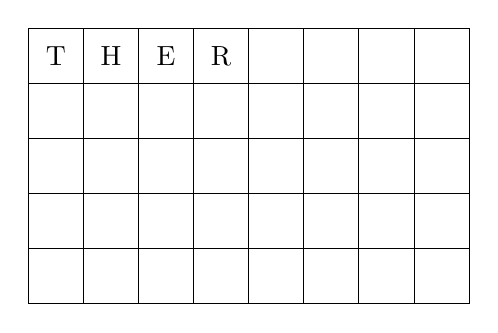
\begin{tikzpicture}[scale = .7]
\draw (0,0) grid (8,5);
\path (.5, 4.5) node {T};
\path (.5+1, 4.5) node {H};
\path (.5+1+1, 4.5) node {E};
\path (.5+1+1+1, 4.5) node {R};

\end{tikzpicture}

\item Now construct the ciphertext by writing down the letters in the columns, in a row. (You can choose to divide up the ciphertext into arbitrary shorter units if you like.)

\vfill

\item Decrypt the phrase 

\so{OIGRM ERDTE OEAGH EFCBI EDSHR NFOPX} 

assuming it was encrypted using a grid with 5 columns (spaces added only to help keep track).
%or abridging the freedom of speech
\be
\item There are 30 letters in the phrase. Since we are using 5 columns, how many rows must there be? \ans

\item Fill in the array down the columns with the ciphertext.
\begin{center}
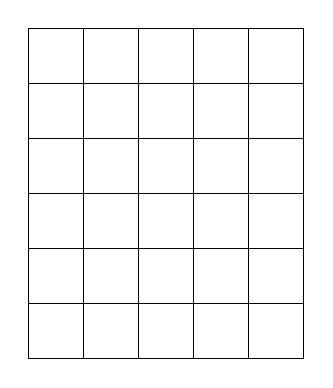
\begin{tikzpicture}[scale = .7]
\draw (0,0) grid (5,6);
\end{tikzpicture}
\end{center}


\item Now decrypt the message by reading across the rows.

\vfill
\ee

\ee

\newpage

\item Next, we will encrypt a phrase using a {\bf keyword} which tells us how to mix up the columns.

Consider the following plaintext:

\so{OR PROHIBITING THE FREE EXERCISE THEREOF}

\be
\item The plaintext has 35 letters (excluding spaces). How many rows are necessary if there are 6 columns? \ans \ How many extra letters will be needed? \ans

\item Write the plaintext in the rows under the key word in the left-hand grid.  Add some extra letters to complete the final row.

\item Rewrite the letters in the keyword RIGHTS so that the letters are in order from earliest alphabetically to latest: \ans[2in]

\item Rewrite those letters in the new order on the top row of the right-hand grid, and fill in the corresponding columns from the left-hand grid.

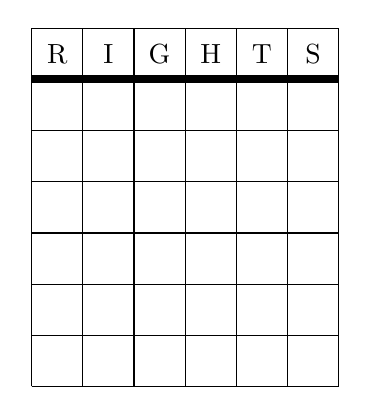
\begin{tikzpicture}[scale = .65]
\draw (0,0) grid (6,7);
\draw[line width = 1mm] (0,6) -- (6,6);
\path (.5, 6.5) node {R};
\path (.5+1, 6.5) node {I};
\path (.5+1+1, 6.5) node {G};
\path (.5+1+1+1, 6.5) node {H};
\path (.5+1+1+1+1, 6.5) node {T};
\path (.5+1+1+1+1+1, 6.5) node {S};
\end{tikzpicture}
\hfill
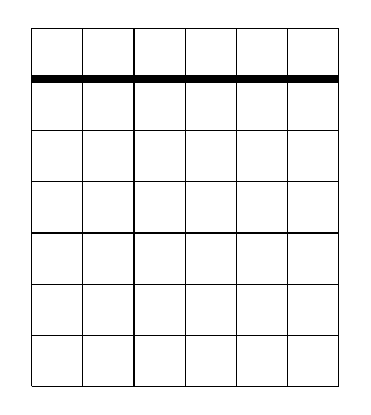
\begin{tikzpicture}[scale = .65]
\draw (0,0) grid (6,7);
\draw[line width = 1mm] (0,6) -- (6,6);
%\path (.5, 6.5) node {R};
%\path (.5+1, 6.5) node {I};
%\path (.5+1+1, 6.5) node {G};
%\path (.5+1+1+1, 6.5) node {H};
%\path (.5+1+1+1+1, 6.5) node {T};
%\path (.5+1+1+1+1+1, 6.5) node {S};
\end{tikzpicture}

\item Now produce your ciphertext by reading down the columns from left to right using the right-hand grid.
\vfill

\ee

\item Using the same keyword RIGHTS, undo the previous process to decrypt the following message, which is 24 characters long. It has been separated into groups of 5 to make it easier to see, not because those are the word lengths.

%\so{CEHTUXEBABIXXVSOQXEILNEDSILREXSALERX}

\so{EOLYR FBXHT ARTHI UGRJX ITYX}

%the right of trial by jury


\be
\item How many rows will you need? \ans Fill in your sorted keyword on the top row of the right grid and then fill in your ciphertext down the columns.
\item Then transfer the columns to your left-hand grid and read off the plaintext in the rows.

%The enumeration in the Constitution, of certain rights



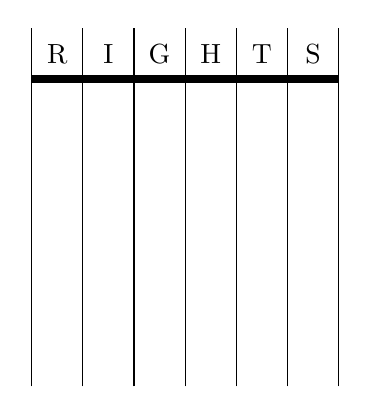
\begin{tikzpicture}[scale = .65]
%\draw (0,0) grid (6,7);
\foreach \i in {0,1,...,6}{\draw (\i,0) -- (\i,7);}
\draw[line width = 1mm] (0,6) -- (6,6);
\path (.5, 6.5) node {R};
\path (.5+1, 6.5) node {I};
\path (.5+1+1, 6.5) node {G};
\path (.5+1+1+1, 6.5) node {H};
\path (.5+1+1+1+1, 6.5) node {T};
\path (.5+1+1+1+1+1, 6.5) node {S};
\end{tikzpicture}
\hfill
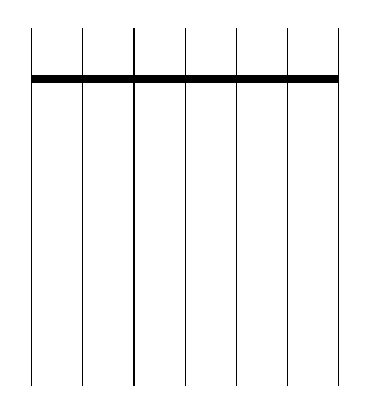
\begin{tikzpicture}[scale = .65]
%\draw (0,0) grid (6,7);
\foreach \i in {0,1,...,6}{\draw (\i,0) -- (\i,7);}
\draw[line width = 1mm] (0,6) -- (6,6);
%\path (.5, 6.5) node {R};
%\path (.5+1, 6.5) node {I};
%\path (.5+1+1, 6.5) node {G};
%\path (.5+1+1+1, 6.5) node {H};
%\path (.5+1+1+1+1, 6.5) node {T};
%\path (.5+1+1+1+1+1, 6.5) node {S};
\end{tikzpicture}

\item What is the plaintext?

\vfill
\ee
\end{enumerate}
\end{document}

%-------------------------------------------------------------------------------------------------------------------------------------------------------------------------------------------------------------------

%%% Local Variables:
%%% mode: latex
%%% TeX-master: t
%%% End:
